\usetikzlibrary {arrows.meta} 
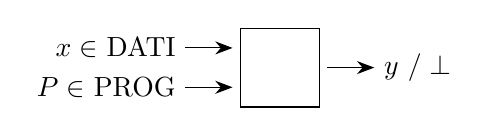
\begin{tikzpicture}

    \draw[-{Stealth[length=2.2mm]}] (2.3,1.75) node[left]{$x\in$\ DATI} -- (2.9,1.75);
    \draw[-{Stealth[length=2.2mm]}] (2.3,1.25) node[left]{$P\in$\ PROG} -- (2.9,1.25);
    \draw (3,2) rectangle (4,1);
    \node at (3.45,1.5) {$\C$};
    \draw[-{Stealth[length=2.2mm]}] (4.1,1.5) -- (4.7,1.5)
        node [right] {$y\ /\perp$};

\end{tikzpicture}